%---------------------------------------%
\section{O que é Ciência Aberta?}
\label{section:openscience}
%---------------------------------------%

%A Ciência sempre se pautou pela disseminação do conhecimento, com destaque para o método científico e a reprodutibilidade de experimentos. 

%A Ciência Aberta parte do pressuposto de que a Ciência é um bem comum, e que todos os insumos, processos e resultados associados a alguma atividade de pesquisa devem ser públicos e abertos a todos os atores sociais, respeitando-se restrições éticas e legais.

O \RSw desempenha um papel central na Ciência Aberta, seja como parte do método científico ou como um de seus resultados~\cite{training:handbook}.
%E o que é a Ciência Aberta?
Nesta seção, apresentamos uma definição para Ciência Aberta e os conceitos mais relevantes para contextualizar o \RS, dentre eles, \textit{Dados Abertos}, \textit{Acesso Aberto}, \textit{Revisão por Pares Aberta}, \textit{Pesquisa Reprodutível Aberta} e \textit{Código Aberto}. 

\subsection{Definição}

A Recomendação da UNESCO sobre Ciência Aberta~\cite{unesco:2021} a define como  ``um  construto  inclusivo  que  combina  vários  movimentos  e  práticas  que  têm  o  objetivo  de   disponibilizar   abertamente   conhecimento   científico   multilíngue,   torná-lo  acessível  e  reutilizável  para  todos,  aumentar  as  colaborações  científicas  e  o  compartilhamento de informações para o benefício da ciência e da sociedade, e abrir os processos de criação, avaliação e comunicação do conhecimento científico a atores da sociedade, além da comunidade científica tradicional''. 

Na definição da UNESCO, a Ciência Aberta abrange todas as disciplinas científicas e todos os aspectos das práticas acadêmicas, incluindo ciências básicas e aplicadas, ciências naturais, sociais e humanas,
e está estruturada sobre quatro pilares (Figura~\ref{fig:unesco}): 
conhecimento científico aberto, infraestrutura científica aberta,  envolvimento aberto dos atores sociais e diálogo aberto com outros sistemas de conhecimento.

\begin{figure}[htbp]
    \centering
    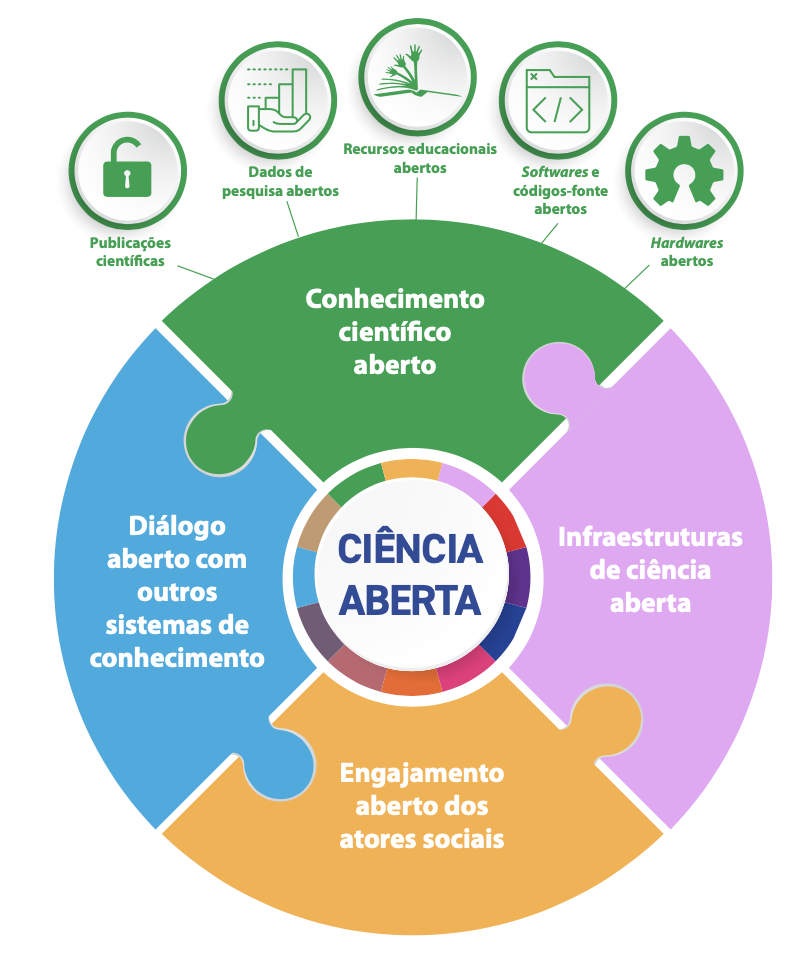
\includegraphics[scale=0.6]{JAI 2023/figures/unesco_OS.png}
    \caption{Definição de Ciência Aberta~\cite{unesco:2021}.}
    \label{fig:unesco}
\end{figure}

No contexto deste capítulo, que trata especificamente sobre princípios e práticas do \RS, colocamos ênfase em conceitos do \textit{conhecimento científico aberto}, que versa sobre o 
acesso aberto a publicações científicas, dados de pesquisa, software de pesquisa, que estejam disponíveis em domínio público ou sob direitos autorais e licenciados sob uma licença aberta. Conceitos relacionados aos demais pilares estão descritos na Recomendação da UNESCO sobre Ciência Aberta~\cite{unesco:2021}.

Consideramos que o termo \textit{Ciência Aberta} designa a \textit{prática da Ciência} de forma que outros possam \textit{colaborar e contribuir}, onde publicações, dados, software e outros artefatos de pesquisa estão \textit{disponíveis online e gratuitamente}, com base em termos que permitem a reutilização, redistribuição e \textit{reprodução} da pesquisa, seus dados e métodos subjacentes.
%
%A Figura~\ref{fig:open-science-map-by-foster} ilustra uma taxonomia que evidencia alguns tópicos e conceitos importantes para Ciência Aberta~\cite{pontika:2015}.

%\begin{figure}[htb]
%    \centering
%    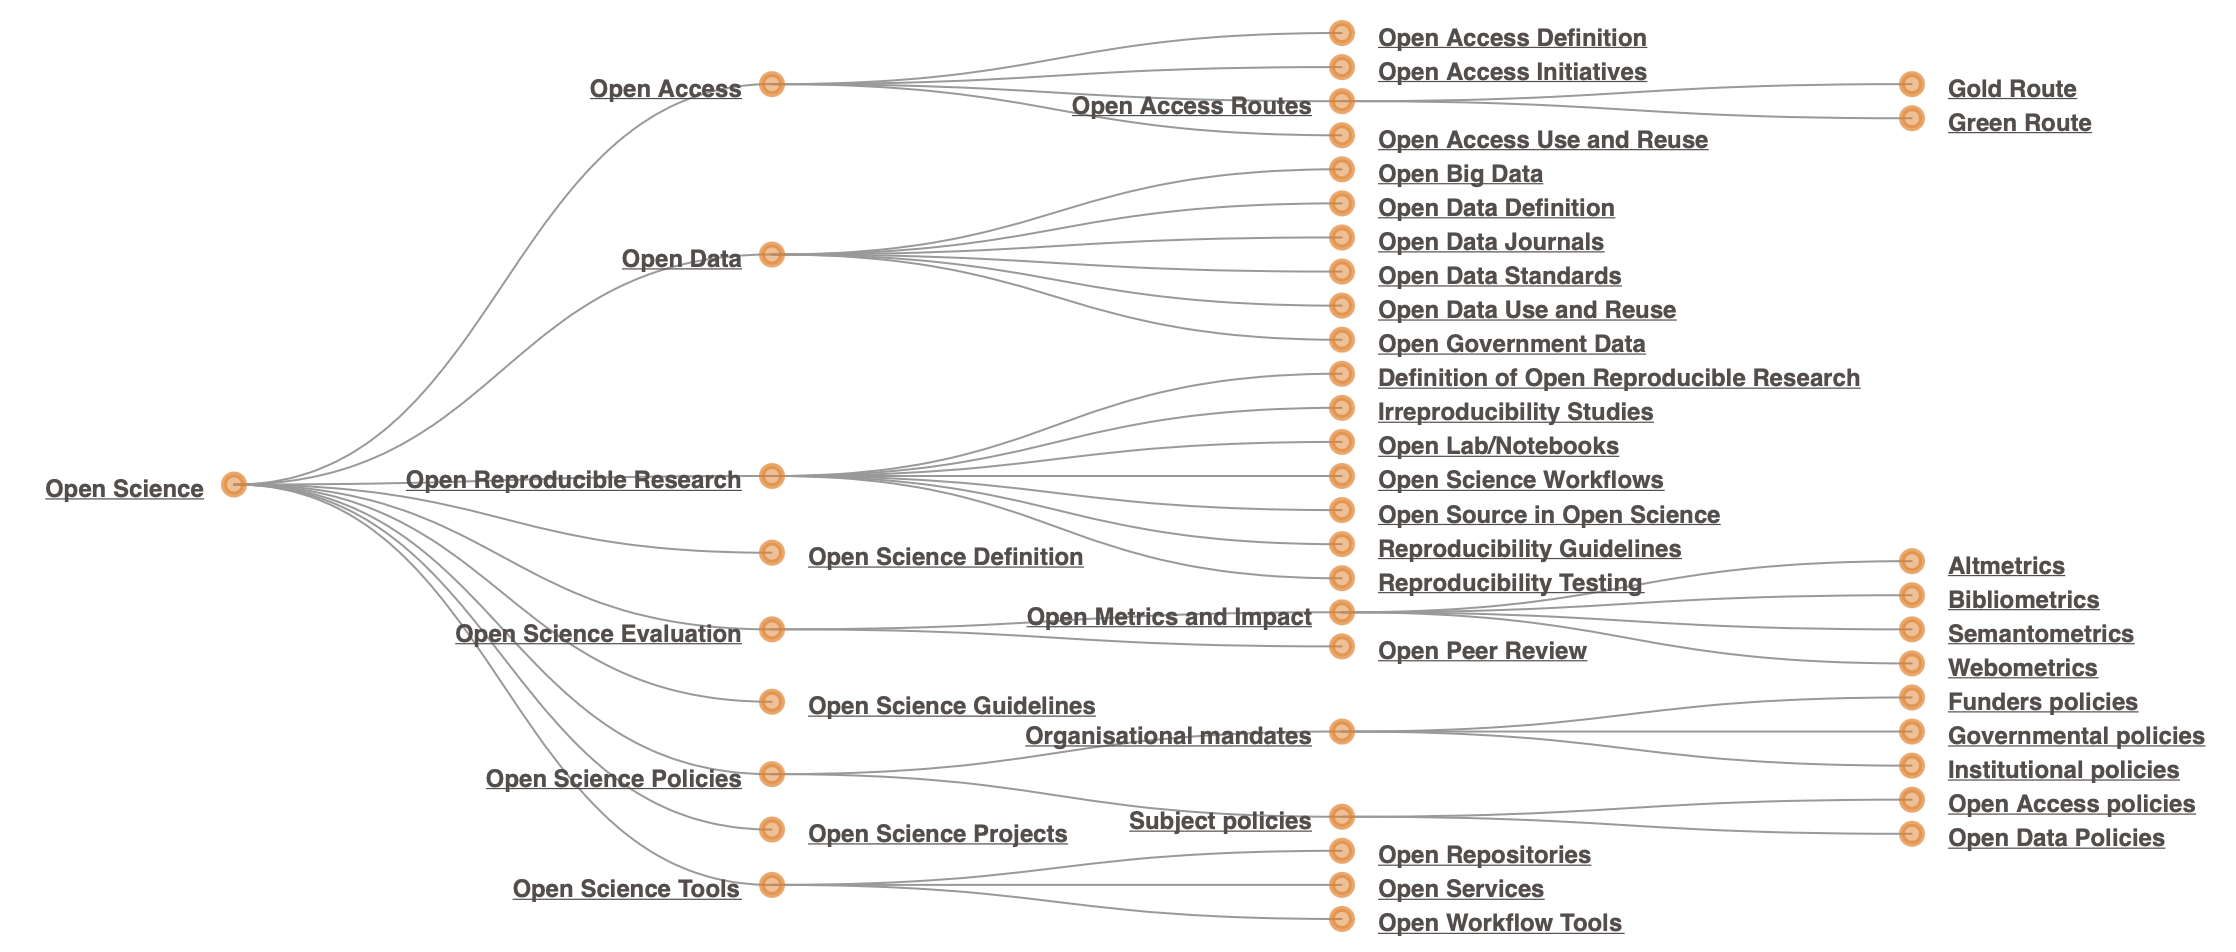
\includegraphics[scale=0.38]{JAI 2023/figures/open-science-map-by-foster.png}
%    \caption{Uma Taxonomia para a Ciência Aberta \cite{pontika:2015}.}
%    \label{fig:open-science-map-by-foster}
%\end{figure}

%Ciência Aberta no Brasil \url{https://www.unesco.org/en/fieldoffice/brasilia/expertise/open-science-brazil}

%------------------------------------------------%
%\subsection{Conceitos}

\subsection{Dados Abertos}

% Open data implies freedom to access, use and re-use for any purpose
Dados abertos estão acessíveis e disponíveis online, gratuitamente e podem ser usados, reutilizados e distribuídos desde que a fonte de dados seja atribuída.
%
Pesquisadores podem depositar os dados de sua pesquisa em um \textit{repositório de dados aberto}, para que outros possam encontrar, utilizar e construir sobre o seu trabalho~\cite{training:handbook}.
%
\textit{Metadados} ou informações sobre os dados, tais como, criador, palavras-chave, unidades, são essenciais para facilitar a descoberta de dados e 
\textit{identificadores permanentes} (PIDs) são necessários para rastrear os dados.

Um \textit{identificador de objeto digital} (DOI) é um identificador exclusivo atribuído a um conjunto de dados para garantir que os dados não sejam perdidos ou identificados incorretamente.
O DOI facilita a citação e o rastreamento do impacto dos conjuntos de dados, assim como os artigos de periódicos citados.
%
A \textit{citação de dados} deve ser considerada tão importante quanto a citação de artigos de periódicos e outros documentos científicos. 
Em geral, uma citação de dados deve incluir nome do autor/criador, data de publicação e título do conjunto de dados,  editora/organizador e DOI.

Agências de fomento à pesquisa passaram a exigir que dados coletados ou criados em projetos financiados sejam compartilhados com a comunidade em geral.
No Brasil, a Fundação de Amparo à Pesquisa do Estado de São Paulo (FAPESP) lançou as bases para a abertura de dados com a exigência, a partir do final de 2017, de Planos de Gestão de Dados quando da submissão de projetos\footnote{\url{https://fapesp.br/gestaodedados}}.

% criou um Código de Boas Práticas em Pesquisa, que, dentre outras determinações, destaca a necessidade da abertura dos procedimentos e resultados da pesquisa financiada pela Fundação, especialmente o ``registro, conservação e acessibilidade de dados e informações'', sempre considerando questões éticas ou legais

Em geral, a organização de dados de pesquisa abertos é temática. 
O World Ocean Database (WOD)\footnote{\url{https://www.ncei.noaa.gov/products/world-ocean-database}} é a maior coleção do mundo de dados abertos de perfis oceânicos uniformemente formatados, com controle de qualidade e disponíveis ao público. Os conjuntos de dados (\textit{datasets}) submetidos recebem um número de acesso (\textit{Accession Number}). Usuários podem utilizar o número de acesso para consultar o Geoportal do \textit{National Centers for Environmental Information (NCEI)} e obter uma cópia exata dos dados originais e seus metadados.

%Boyer, T.P., O.K. Baranova, C. Coleman, H.E. Garcia, A. Grodsky, R.A. Locarnini, A.V. Mishonov, C.R. Paver, J.R. Reagan, D. Seidov, I.V. Smolyar, K. Weathers, M.M. Zweng,(2018): World Ocean Database 2018. A.V. Mishonov, Technical Ed., NOAA Atlas NESDIS 87. \url{https://www.ncei.noaa.gov/sites/default/files/2020-04/wod_intro_0.pdf}.

\subsection{Acesso Aberto}

%Acesso online e gratuito a conteúdo científico revisado por pares com direitos autorais limitados e restrições de licenciamento. [FOSTER]

Uma das formas mais comuns de divulgar os resultados de uma pesquisa científica é escrever um artigo e publicá-lo em periódicos, anais de conferências ou livros. 
%
Em geral, tais publicações são disponibilizadas ao público mediante pagamento, através de uma assinatura institucional ou de forma individual. Entretanto, nos últimos anos, as taxas praticadas pelas editoras têm sido altíssimas, inviabilizando o amplo acesso ao conhecimento científico e criando desigualdades regionais.

O Movimento de Acesso Aberto\footnote{\url{https://en.unesco.org/open-access/open-access-movement}} surgiu com o propósito de
tornar todos os resultados de pesquisa disponíveis para o público sem quaisquer restrições. 
As duas estratégias mais conhecidas para publicação de artigos científicos promovem modelos alternativos, visando a ampla divulgação e redução de custos. 

\subsection*{Publicação em repositórios institucionais ou temáticos}

Esta estratégia recomenda o auto-arquivamento por pesquisadores, que depositam e divulgam os seus artigos em repositórios abertos -- institucionais ou temáticos. 
% Estratégia: fornecer ferramentas e assistência aos acadêmicos para o depósito dos seus artigos com revisão por pares em repositórios eletrônicos abertos. 

No Brasil, várias universidades oferecem repositórios institucionais para que pesquisadores depositem a sua produção acadêmica. 
Por exemplo, o Repositório Institucional da Universidade Federal da Bahia (RI-UFBA)\footnote{\url{https://repositorio.ufba.br}} é um serviço de informação científica que utiliza o DSpace\footnote{\url{https://github.com/DSpace}}, um pacote de software livre e de código aberto, para gerenciar e a disseminar a produção acadêmica da UFBA em consonância com as recomendações da Ciência Aberta. 

Nos últimos anos, pesquisadores têm depositado uma versão de seus artigos pré-impressão (\textit{preprints}) em repositórios abertos temáticos, por exemplo, o arXiv\footnote{\url{https://arxiv.org}}. 
O \textit{Computing Research Repository (CoRR) - arXiv}\footnote{\url{https://arxiv.org/archive/cs}} hospeda artigos da área de Computação.

% NÃO - O \textit{Open Science Repository}\footnote{\url{http://www.open-science-repository.com}} é um projeto para publicar trabalhos de pesquisa originais em acesso aberto, o que significa que os leitores não precisam pagar para ter acesso ao conteúdo completo da pesquisa. Pesquisadores de todos os campos da ciência podem publicar artigos originais e outras comunicações acadêmicas.

\subsection*{Publicação em periódicos e revistas de acesso aberto} 

Esta estratégia recomenda o desenvolvimento de uma nova geração de periódicos que usam os direitos de autor e outros instrumentos para garantir o acesso aberto permanente a todos os artigos que publicam. Os periódicos de acesso aberto permitem o acesso gratuito aos leitores e autorizam a reutilização da maioria dos seus conteúdos quase sem restrições.
%
Vários periódicos têm sido criados com acesso aberto, por exemplo, a série \textit{PeerJ}. %\footnote{\url{https://peerj.com}}. 
O periódico \textit{PeerJ Computer Science}\footnote{\url{https://peerj.com/computer-science/}} é o veículo voltado para a área de Computação.

O \textit{Journal of Open Source Software} (JOSS)\footnote{\url{https://joss.theoj.org}}
é um periódico de acesso aberto voltado para a publicação de \textit{pacotes de software de pesquisa}, sem taxas de processamento de artigos ou taxas de assinatura~\cite{joss:2017}.
O JOSS possui um processo formal de revisão por pares para melhorar a qualidade do software submetido. Após a aceitação no JOSS, o artigo recebe um DOI e é listado no site do JOSS.


% Closed access is the traditional form of scientific publishing. In this mode, once an article is published, it no longer belongs to you. You can share article copies privately, but may not make them public. 
%
% Green open access allows you to share either the reviewed (post-print) or originally submitted (pre-print) manuscript of your paper to certain websites or repositories. Often there is an embargo period of 6-24 months before sharing is allowed to give the publisher the chance to recoup its investment (certain journals may also allow sharing the published version after an embargo period). 
%
%Gold open access publishing retains the copyright to the author. This makes the final paper free to download for anyone from the journal website and allows unrestricted sharing online. Since the publisher in this case does not get to charge the reader, it is often the author who has to pay a fee for publishing. There is also a caveat: many closed-access journals offer unrestricted access to a specific article against a fee from the author. This so-called “hybrid gold open-access” mode is not encouraged by many scientific institutions because they essentially have to pay the publisher twice – once for the subscription and on top of it – a publication fee. 

\subsection*{Publicação de Artefatos de Pesquisa}

Além dos artigos científicos, repositórios de acesso aberto também são úteis para preservar e compartilhar \textit{outros produtos e artefatos} gerados durante a pesquisa científica,  permitindo que outros pesquisadores possam estudá-los e trabalhar com eles.
%
Há diversos repositórios abertos internacionais, dentre eles, 
Digital Commons, DSpace e  Wikimedia Commons~\cite{abdo2015direccoes}.
%, EPrints, Dataverse, GenBank, CERN Open Hardware Repository, iGem Registry of Standard Biological Parts, Addgene, Central, EuroBioBank, e Cooperative Human Tissue Network
%No Brasil, há alguns repositórios temáticos, como o SinBiota\footnote{\url{http://sinbiota.biota.org.br/about}}.
%
Exemplos de repositórios abertos conhecidos pela comunidade brasileira são Zenodo, Figshare e OSF.

\textit{Zenodo}\footnote{\url{https://zenodo.org}} é um repositório aberto de uso geral, criado para apoiar os movimentos de acesso aberto e dados abertos na Europa.
Pesquisadores podem depositar artigos, conjuntos de dados, \RS, relatórios e quaisquer outros artefatos digitais relacionados à pesquisa. Para cada envio, um identificador de objeto digital persistente (DOI) é criado, o que torna os itens armazenados facilmente citáveis.
%
\textit{Figshare}\footnote{\url{https://figshare.com}} permite a hospedagem de grandes quantidades de dados que aparecem em artigos online.
%
O \textit{Open Science Framework (OSF)}\footnote{\url{https://osf.io}} é uma ferramenta
de código aberto para o gerenciamento de projetos que oferece suporte aos pesquisadores durante todo o ciclo de vida do projeto de pesquisa. 
É também uma ferramenta de colaboração, que dá suporte ao trabalho em equipe em projetos de forma privada ou torna todo o projeto e seus artefatos publicamente acessíveis para ampla divulgação. 
%OSF permite conexões com outras ferramentas científicas que os pesquisadores usam, agilizando seu processo, aumentando a eficiência e promovendo a transparência e reprodutibilidade científicas.

%provide community resources and capabilities to enable scientists and workflow systems developers to discover software products, related efforts, events, technical reports, etc. and engage in community-wide efforts to tackle workflows grand challenges
% Use collaborative tools such as GitHub and the Open Science Framework for increased collaboration for the research process, writing/authoring, and sharing your research outputs.


%\subsection{Revisão por Pares Aberta}
\begin{comment}
% Peer review is a complex process.
% The main idea behind open peer-review is to enable a fully transparent and author-driven process
% Researchers can use open reviews to their advantage and they can get credit for the reviews they perform

A Revisão por Pares Aberta (\textit{Open Peer Review}) é um processo de validação por pares realizado abertamente na Internet, em que alguns aspectos do processo de revisão são abertos à comunidade de pesquisa ou ao público. Os manuscritos são disponibilizados pelos autores imediatamente antes dos procedimentos formais de revisão por pares. 
No processo, autores e revisores estão cientes da identidade um do outro e os relatórios de revisão são abertos e acessíveis e são publicados juntamente com o artigo disponibilizado. Uma entidade organizacional diferente do local de publicação dá suporte ao processo de revisão.
A comunidade em geral pode contribuir para o processo de revisão (pesquisadores ou o público em geral).
\end{comment}

\subsection{Pesquisa Reprodutível Aberta}

A \textit{Pesquisa Reprodutível Aberta} é definida como ``o ato de praticar Ciência Aberta e a provisão de oferecer aos usuários acesso gratuito a elementos experimentais para reprodução de pesquisas'' \cite{training:handbook}.
%
A Reprodutibilidade é definida como a capacidade de investigadores independentes de tirar as mesmas conclusões de um experimento seguindo a documentação compartilhada pelos pesquisadores que originalmente realizaram a pesquisa.
A reprodutibilidade na pesquisa científica aumenta a credibilidade da pesquisa.

Na pesquisa reprodutível aberta, os dados abertos fornecem os insumos necessários para que os pesquisadores validem e reproduzam os resultados uns dos outros. 
Entretanto, o acesso aos dados de pesquisa e artigos científicos não é mais suficiente para assegurar a reprodutibilidade na pesquisa. 
É importante definir e documentar os fluxos de trabalho (\textit{workflows}) da pesquisa.

O pesquisador deve pensar em reprodutibilidade desde o início de sua pesquisa, documentando e compartilhando cada etapa do fluxo de trabalho -- desde a coleta ou acesso aos dados, filtragem  e limpeza, até a análise de dados -- de modo a criar um roteiro ou guia para que ele e outros pesquisadores possam seguir.  A documentação deve incluir e justificar decisões importantes, por exemplo, excluir certos valores ou ajustar certos parâmetros do modelo.
O uso de software de {\em workflow} permite que cientistas automatizem e repliquem facilmente os fluxos de trabalho
em cada etapa de coleta e análise de dados.

A iniciativa {\em Workflows Community}\footnote{\url{https://workflows.community/}} compartilha recursos fornecidos pela comunidade de plataformas de software de coleta e análise de dados em pesquisa científica. 
%
Ferramentas como o Nextflow\footnote{\url{https://nextflow.io}} orquestram, de maneira simplificada e aberta, {\em pipelines} de dados de maneira portável e escalável, com suporte a instalação em uma variedade de plataformas, incluindo computadores locais,  infrastruturas como HPC e Kubernetes, e de Computação em Nuvem como AWS, Azure e Google Cloud. 
%
Outras soluções, por exemplo, o {\em Guix Workflow Language (GWL)}\footnote{\url{https://guixwl.org}} 
oferecem extensões de apoio a computação científica para a linguagem declarativa de pacotes do GNU Guix, permitindo combinar pacotes Guix com workflows científicos.

Na Ciência Aberta, além dos dados abertos e fluxos de trabalho documentados, o software também é reconhecido como elemento experimental e parte fundamental do método científico.

%-------------------%
\begin{comment}

\begin{table}[tbp]

\begin{tcolorbox}[colback=white,title=Definições da Ciência Aberta]
\begin{description}
    \item[Dados Abertos.] Dados online, gratuitos e acessíveis que podem ser usados, reutilizados e distribuídos desde que a fonte de dados seja atribuída.
\end{description}
\begin{description}
    \item[Acesso Aberto.] Acesso online e gratuito a conteúdo científico revisado por pares com direitos autorais limitados e restrições de licenciamento.
%    \item[Revisão por pares Aberta.] Processo de validação por pares realizado abertamente na Internet.
    \item[Código Aberto.]
    Software amplamente acessível para uso, seja como software livre, gratuito ou comercial.
    \item[Software Livre.]
    Software disponibilizado com licenças atribuídas que permitem ao usuário leitura, execução, adaptação e distribuição.
    \item[Pesquisa Reprodutível Aberta.]  
    Ato de praticar Ciência Aberta e oferecer acesso gratuito a elementos experimentais para reprodução de pesquisas.
\end{description}
\end{tcolorbox}

\end{table}
\end{comment}

%-------------------------------------%

\subsection{Código Aberto}

Na Ciência Aberta, 
\textit{Código Aberto} é o termo usado para caracterizar software amplamente acessível para uso, seja como software livre, gratuito ou comercial~\cite{training:handbook}.
%
``Aberto'' pode ter dois significados diferentes: apenas o código-fonte está disponível em código aberto ou o software é desenvolvido de forma aberta~\cite{herman:2022}.

Projetos de Software Livre disponibilizam o código-fonte e são 
desenvolvidos de forma aberta, com licenças de software atribuídas que permitem ao usuário leitura, execução, adaptação e distribuição.
%
Alguns pesquisadores consideram que o software livre é um pré-requisito para a Ciência Aberta~\cite{flach:sbc:2021,10.12688/f1000research.23224.2}.

Uma outra forma de compartilhar código aberto são os \textit{notebooks}, fundamentados na Programação Letrada (\textit{Literate Programming})~\cite{knuth:84}). 
Um programa letrado é uma combinação de documentação e programa-fonte organizada de modo que possa ser lida por pessoas.
Ferramentas de programação letrada extraem do arquivo uma documentação legível e um programa-fonte compilável. 
\textit{Notebooks} Jupyter\footnote{\url{https://jupyter.org}} são usados para análise exploratória e preparação de dados, treinamento e teste dos modelos. O código escrito em um \textit{notebook} pode ser extraído e empacotado como um módulo ou biblioteca Python para posterior reutilização.

% The notebooks on GitHub are the actual ‘scholarship’
%sharing the code through interactive notebooks,
%a browser-based and interactive notebook with support for code, rich text, mathematical expressions, inline plots and other rich media
%an ideal platform to support open and reproducible research.
%- The notebooks on GitHub are the actual ‘scholarship’

% Considere usar ferramentas de código aberto. Isso permite que qualquer pessoa reproduza pesquisas com mais facilidade, e ajuda a identificar quem tem a licença certa para o software usado.

%Diferentemente de desenvolvedores de software comercial tradicionais, provavelmente alinhados com desenvolvedores em projetos de código aberto, os programadores de software aberto não têm clientes e os requisitos do software raramente são congelados.




%------------------------%

% to provide guidance to the research enterprise and its stakeholders as they build strategies for achieving open science and take the next steps. In order to frame the issues and possible actions, the committee developed the concept of open science by design, defined as a set of principles and practices that fosters openness throughout the entire research life cycle
%National Academies of Sciences, Engineering, and Medicine. 2018. Open Science by Design: Realizing a Vision for 21st Century Research. Washington, DC: The National Academies Press. https://doi.org/10.17226/25116.

%In recent years “Alternative Metrics” or altmetrics have become a topic in the debate about a balanced assessment of research efforts that complement citation counting by gauging other online measures of research impact, including bookmarks, links, blog posts, tweets, likes, shares, press coverage and the like.

%Normalmente, um “projeto” no OSF, ou em qualquer outro repositório, será associado a um ou mais estudos conforme relatado em um artigo. A estrutura da pasta dependerá naturalmente do que você deseja compartilhar. Não existe um padrão comumente aceito. As pastas podem, por exemplo, ser organizadas por estudo, por tipo de arquivo (scripts de análise, dados, materiais, papel) ou tipo de dados (bruto x processado).

